\section{Experimental Results}  \label{sec:exp}

\subsection{Experimental Setup}

\subsubsection{Datasets}

\paragraph*{Berkeley Dataset}

The Intel Berkeley Research lab dataset~\cite{berkeley2004lab} records temperature, humidity, light, and voltage for 54 sensors (with 1 missing completely missing) for which locations are given (see Figure \ref{berkeley_lab}).
The dataset includes 2.3M sensor observations and was recorded between February 28th and April 5th, 2004 in an indoor lab environment.

\begin{figure}[H]
\centering
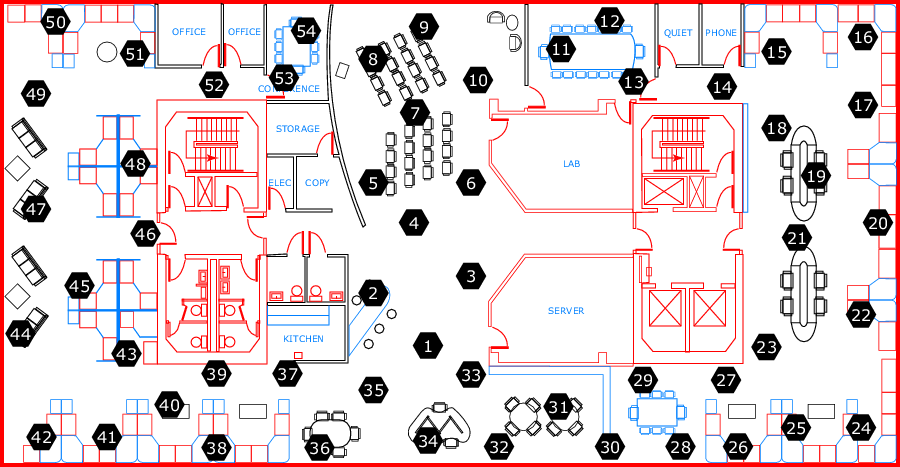
\includegraphics[scale=0.25]{berkeley_lab.png}
\caption{Intel Berkeley Research Lab Floorplan} \label{berkeley_lab}
\end{figure}

Outlier Filtering : Observation removed if temperature $> 100\degc$, temperature $< 5\degc$, or humidity $< 16\%$.

Gridding : Dataset falls on even 30s grid points for the first 10000 time steps (which is all we consider), so no gridding need be performed.

\paragraph*{Traffic Dataset}

The Traffic Dataset records the temperature, humidity, and voltage conditions of 20 sensor nodes and one gateway node.
This dataset, collected by the Bio-industrial Department at National Taiwan University, was recorded over a 2.5 year time period ending in 2011 in an outdoor location high traffic area in Taipei, Taiwan.

\begin{figure}[H]
\centering
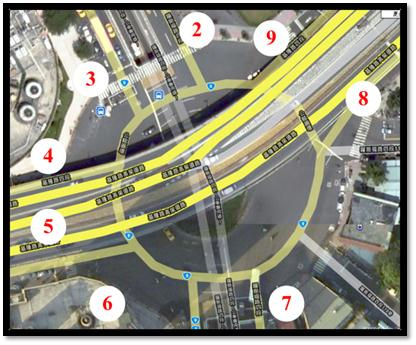
\includegraphics[scale=0.5]{traffic_wsn.png}
\caption{Traffic Sensor Deployment Configuration (7 sensors of 20 shown)}
\end{figure}

Outlier Filtering : \redtext{this was done by chung-yi.. please fill this in!}

Gridding : The original dataset recorded most readings at around the xx:03 and xx:33 minute marks, so a 6 min window centered at
these points captured the data for 30min internal readings. Where more than one reading was recorded for a given node
within within a given window, the closest to the 3 or 33 min mark was chosen.

\subsubsection{Dataset Preparation}

\paragraph*{Common Methodology}

Datasets of various lengths are produced from the single input dataset for our experiments, namely 2500, 5000, and 10000.
There is an initially missing portion of the observations which can be considered Missing At Random (MAR).
To this, we impose two different types of Missing Completely At Random (MCAR) sampling techniques to build validation and testing datasets.

\paragraph*{Random Missing Pattern}

This pattern reflects choosing a random time and random sensor to be missing and hence removed from the training set.
We define three values $a, b, c$ as follows.

\begin{itemize}
\item $b\%$ of the non-missing data is randomly selected (without replacement) to be the validation set
\item $c\%$ of the non-missing data is randomly selected (without replacement) to be the testing set
\item The remaining data is part of the training set (this would be $a\%$ of the total data given no missing; assuming missing rate of $\%m$, the actual data in training set is $100-\%a-\%b-\%m$
\end{itemize}

\paragraph*{Temporal Missing Pattern}

This pattern reflects testing the effect of all data missing after a certain point in time.
We define three values $a, b, c$ as follows.

\begin{itemize}
\item Here, we have the last $c\%$ of time is in test and the prior $b\%$ to test is the validation.
\item A total of 10 sensors are ``covered up'' in the validation and testing: 2,4,6,8,10,14,17,19,20,99
\end{itemize}

\subsection{Basic Experimental Results} %from Chung-Yi

%validation setting
We implemented linear interpolation~(LI), TRMF, Hybrid-kNN, DESM, STI and conducted experiment on the two data sets.

\subsubsection{Random Split}
\textbf{Table \ref{table:berkeley_random_hum}, \ref{table:berkeley_random_light} and \ref{table:berkeley_random_tem}} show the result of random split on Berkeley data set. It is clear that TRMF outperforms others in all cases. Yet, linear interpolation is quite competitive when the size of testing set is small, since the sampling rate of Berkeley data set is fairly high, and the temporal correlation is prominent in this data set.  

\textbf{Table \ref{table:traffic_random_hum} and \ref{table:traffic_random_tem}} show the result of random split on traffic data set. The DESM and STI are not included since they perform badly and the location information of the sensor nodes is not available in this data set. Again, TRMF outperforms other models in all cases. However, the performance of linear interpolation deteriorates a lot and this corresponds to the low sampling rate in traffic data set. 

In short, we believe TRMF successfully combines and leverages the temporal correlation and spatial correlation of the sensors, so it achieves the best performance. %hybrid???

\begin{table}[htbp]
\centering
\caption{RMSE of (Berkeley, random, humidity)}
\label{table:berkeley_random_hum}
\begin{tabular}{ r | r r r r r}
	testing	&LI	&TRMF	&H-kNN	&DESM	&STI\\ \hline
	85\%	&0.3187	&0.1943	&0.3544	&1.9574	&1.2196\\ 
	80\%	&0.1711	&0.1420	&0.2640	&0.5444	&1.2203\\
	70\%	&0.1266	&0.1138	&0.2437	&0.3178	&1.4724\\
	50\%	&0.0950	&0.0916	&0.1993	&0.2190	&1.6481\\
	30\%	&0.0845	&0.0815	&0.1812	&0.1804	&1.6495\\
	10\%	&0.0750	&0.0758	&0.1267	&0.1599	&1.6039\\
	 5\%	&0.0742	&0.0750	&0.1208	&0.1480	&1.5493
\end{tabular}
\end{table}

\begin{table} [htbp]
\centering
\caption{RMSE of (Berkeley, random, light)}
\label{table:berkeley_random_light}
\begin{tabular}{ r | r r r r r}
	testing	&LI	&TRMF	&H-kNN	&DESM	&STI\\ \hline
	85\%	&70.81	&50.01	&74.76	&18,531.37	&225.62\\
	80\%	&52.94	&34.67	&61.22	&6,250.40	&258.23\\
	70\%	&38.71	&27.51	&52.96	&215.88	&311.00\\
	50\%	&29.89	&21.58	&41.38	&356.69	&356.31\\
	30\%	&25.04	&17.21	&33.67	&112.57	&366.87\\
	10\%	&23.89	&17.85	&27.94	&41.72	&363.34\\
	 5\%	&20.85	&14.40	&24.34	&44.35	&354.17
\end{tabular}
\end{table}

\begin{table}[htbp]
\centering
\caption{RMSE of (Berkeley, random, temperature)}
\label{table:berkeley_random_tem}
\begin{tabular}{ r | r r r r r}
	testing	&LI	&TRMF	&H-kNN	&DESM	&STI\\ \hline
	85\%	&0.1673	&0.1140	&0.1914	&1.0886	&0.5537\\
	80\%	&0.0705	&0.0452	&0.1119	&0.2977	&0.5064\\
	70\%	&0.0415	&0.0316	&0.1113	&0.1668	&0.5835\\
	50\%	&0.0270	&0.0230	&0.0802	&0.0954	&0.6443\\
	30\%	&0.0206	&0.0182	&0.0529	&0.0665	&0.6375\\
	10\%	&0.0162	&0.0152	&0.0429	&0.0481	&0.6113\\
	 5\%	&0.0187	&0.0157	&0.0342	&0.0478	&0.5930
\end{tabular}
\end{table}

\begin{table} [htbp]
\centering
\caption{RMSE of (traffic, random, humidity)}
\label{table:traffic_random_hum}
\begin{tabular}{ r | r r r r r}
	testing	&LI	&TRMF	&Hybrid-kNN \\ \hline
	85\%	&15.7250	&4.6898	&11.8941\\ 
	80\%	&11.6299	&3.5391	&7.3071\\
	70\%	& 7.2693	&2.5865	&4.5587\\
	50\%	& 4.2328	&1.9503	&3.4578\\
	30\%	& 3.1837	&1.6748	&2.9011\\
	10\%	& 2.6897	&1.5707	&2.5107\\
	 5\%	& 2.5880	&1.5098	&2.4012
\end{tabular}
\end{table}

\begin{table} [htbp]
\centering
\caption{RMSE of (traffic, random, temperature)}
\label{table:traffic_random_tem}
\begin{tabular}{ r | r r r r r}
	testing	&LI	&TRMF	&Hybrid-kNN \\ \hline
	85\%	&5.3057	&1.6235	&4.0140\\ 
	80\%	&4.0000	&1.2159	&2.5090\\
	70\%	&2.5084	&0.9017	&1.5385\\
	50\%	&1.4770	&0.6898	&1.1923\\
	30\%	&1.1011	&0.5865	&1.0046\\
	10\%	&0.9376	&0.5521	&0.8849\\
	 5\%	&0.9149	&0.5196	&0.8663
\end{tabular}
\end{table}

\subsubsection{Temporal Split}
\textbf{Table \ref{table:berkeley_temporal_hum}, \ref{table:berkeley_temporal_light} and \ref{table:berkeley_temporal_tem}} show the result of random split on Berkeley data set and \textbf{Table \ref{table:traffic_temporal_hum} and \ref{table:traffic_temporal_tem}} show the result of random split on traffic data set.
In the temporal split, it is clear that linear interpolation performs terribly since its prediction is simply the last reading of the sensor.

\begin{table}[htbp]
\centering
\caption{RMSE of (Berkeley, temporal, humidity)}
\label{table:berkeley_temporal_hum}
\begin{tabular}{ r | r r r r r}
	testing	&LI	&TRMF	&H-kNN	&DESM	&STI\\ \hline
	85\%	&3.9669	&1.1250	&1.4492	&3.9682	&0.7876\\ 
	80\%	&4.1829	&1.0069	&1.6694	&4.1853	&0.7918\\
	70\%	&5.4211	&1.2549	&0.9690	&5.4217	&0.8651\\
	50\%	&6.4429	&0.8844	&1.0252	&6.4431	&0.9612\\
	30\%	&2.2225	&0.9314	&0.9280	&2.2335	&0.8643\\
	10\%	&1.2076	&0.5392	&0.6358	&1.2165	&0.6878\\
	 5\%	&2.3060	&0.4285	&0.7768	&2.3077	&0.7960
\end{tabular}
\end{table}

\begin{table}[htbp]
\centering
\caption{RMSE of (Berkeley, temporal, light)}
\label{table:berkeley_temporal_light}
\begin{tabular}{ r | r r r r r}
	testing	&LI	&TRMF	&H-kNN	&DESM	&STI\\ \hline
	85\%	&330.55	&176.51	&196.39	&330.85	&251.32\\ 
	80\%	&320.02	&166.79	&239.09	&320.00	&251.35\\
	70\%	&497.84	&120.53	&257.11	&499.70	&206.58\\
	50\%	&194.54	&58.39	&68.55	&195.17	&208.28\\
	30\%	&312.10	&33.83	&77.45	&312.12	&289.20\\
	10\%	&293.47	&20.60	&84.89	&293.87	&213.90\\
	 5\%	&277.85	&7.81	&79.05	&280.36	& 92.72
\end{tabular}
\end{table}


\begin{table}[htbp]
\centering
\caption{RMSE of (Berkeley, temporal, temperature)}
\label{table:berkeley_temporal_tem}
\begin{tabular}{ r | r r r r r}
	testing	&LI	&TRMF	&H-kNN	&DESM	&STI\\ \hline
	85\%	&3.0873	&0.6098	&0.5312	&3.0876	&0.4786\\ 
	80\%	&3.7602	&0.6221	&0.5136	&3.7606	&0.4921\\
	70\%	&2.3195	&0.4429	&0.4058	&2.3214	&0.4152\\
	50\%	&3.5948	&0.3029	&0.3037	&3.5952	&0.4859\\
	30\%	&1.9598	&0.2247	&0.3402	&1.9615	&0.5322\\
	10\%	&0.8870	&0.2364	&0.2796	&0.8941	&0.3263\\
	 5\%	&1.0241	&0.0853	&0.3047	&1.0156	&0.3506
\end{tabular}
\end{table}

\begin{table} [htbp]
\centering
\caption{RMSE of (traffic, temporal, humidity)}
\label{table:traffic_temporal_hum}
\begin{tabular}{ r | r r r r r}
	testing	&LI	&TRMF	&Hybrid-kNN \\ \hline
	85\%	&16.6428	&5.3882	&5.3955\\ 
	80\%	&27.7509	&5.0636	&5.0810\\
	70\%	&21.4693	&5.5701	&5.0198\\
	50\%	&25.8277	&5.8469	&5.1926\\
	30\%	&27.4891	&5.0048	&5.0268\\
	10\%	&18.9358	&4.6402	&4.1944\\
	 5\%	&23.5126	&4.0820	&3.6661
\end{tabular}
\end{table}


\begin{table} [htbp]
\centering
\caption{RMSE of (traffic, temporal, temperture)}
\label{table:traffic_temporal_tem}
\begin{tabular}{ r | r r r r r}
	testing	&LI	&TRMF	&Hybrid-kNN \\ \hline
	85\%	& 8.6774	&2.0011	&1.8381\\ 
	80\%	&11.4353	&1.5281	&1.6787\\
	70\%	& 7.1857	&1.8447	&1.6644\\
	50\%	&10.5938	&1.7748	&1.5793\\
	30\%	&14.1343	&1.6737	&1.6874\\
	10\%	&16.1660	&1.4345	&1.4137\\
	 5\%	&10.0223	&1.4254	&1.3560
\end{tabular}
\end{table}

\subsubsection{Multivariate TRMF}
We see substantial improvement (if look at all to help) 

\begin{table}[htbp]
\caption{Multivariate TRMF on Traffic Data Set}
\label{traffic}
\begin{tabular}{r | r r r}
traffic dataset	&TRMF	&MtMF	&MtMF-all \\ \hline
humid 5-10-85	&4.6898	&4.6690	&3.0966\\
humid10-10-80	&3.5391	&3.5232	&2.3081\\
humid20-10-70	&2.5865	&2.5886	&1.8027\\
humid40-10-50	&1.9503	&1.9435	&1.5207\\
humid60-10-30	&1.6748	&1.6594	&1.4116\\
humid80-10-10	&1.5707	&1.5574	&1.3706\\
humid85-10- 5	&1.5098	&1.4963	&1.3301\\
 temp 5-10-85	&1.6235	&1.6105	&0.9620\\
 temp10-10-80	&1.2159	&1.2186	&0.7305\\
 temp20-10-70	&0.9017	&0.8936	&0.6002\\
 temp40-10-50	&0.6898	&0.6819	&0.5200\\
 temp60-10-30	&0.5865	&0.5818	&0.4770\\
 temp80-10-10	&0.5521	&0.5464	&0.4652\\
 temp85-10- 5	&0.5196	&0.5126	&0.4319\\
humid 5-10-85t	&5.3882	&5.3994	&5.1394\\
humid10-10-80t	&5.0636	&5.2424	&4.2964\\
humid20-10-70t	&5.5701	&5.6727	&4.2332\\
humid40-10-50t	&5.8469	&6.0046	&4.6036\\
humid60-10-30t	&5.0048	&4.9566	&3.7443\\
humid80-10-10t	&4.6402	&4.7294	&3.2574\\
humid85-10- 5t	&4.0820	&3.9843	&3.1709\\
 temp 5-10-85t	&2.0011	&2.0344	&1.5952\\
 temp10-10-80t	&1.5281	&1.7150	&1.2174\\
 temp20-10-70t	&1.8447	&1.9223	&1.1501\\
 temp40-10-50t	&1.7748	&1.7961	&1.0494\\
 temp60-10-30t	&1.6737	&1.6819	&1.2274\\
 temp80-10-10t	&1.4345	&1.4225	&0.9267\\
 temp85-10- 5t	&1.4254	&1.3374	&0.9259

\end{tabular}
\end{table}

\begin{table}[htbp]
\caption{Multivariate TRMF on Berkeley Data Set, random}
\label{traffic}
\begin{tabular}{r | r r r}
berkeley dataset	&TRMF	&MtMF	&MtMF-all \\ \hline
humid  5 &0.1936	&0.1941	&0.1594\\
humid 10 &0.1424	&0.1421	&0.1219\\
humid 20 &0.1140	&0.1139	&0.0975\\
humid 40 &0.0918	&0.0910	&0.0824\\
humid 60 &0.0815	&0.0808	&0.0762\\
humid 80 &0.0756	&0.0749	&0.0712\\
humid 85 &0.0750	&0.0740	&0.0713\\
 temp  5 &0.1136	&0.1158	&0.0694\\
 temp 10 &0.0454	&0.0482	&0.0371\\
 temp 20 &0.0316	&0.0329	&0.0264\\
 temp 40 &0.0232	&0.0233	&0.0201\\
 temp 60 &0.0181	&0.0183	&0.0166\\
 temp 80 &0.0155	&0.0155	&0.0144\\
 temp 85 &0.0158	&0.0159	&0.0142
\end{tabular}
\end{table}
\subsection{Heterogeneous Signal Incorporation}

We compare our TF method with the models without modeling heterogeneous sensor correlations in this section.
The Tensor Factorization naturally allow us to add additional nominal dimensions to the model, e.g.\ node id or sensor coordinates.
The three-order TF is used in the experiment, each dimension represent node id, time frame number and heterogeneous signal.  
Due to the indexes of each dimension are discrete, the heterogeneous sensor data are not able directly used.
Therefore, the discretization of heterogeneous data is needed.
Before training, the heterogeneous signal are divide into some bins according to the value.
Each bin represents the index of the dimension.
Table ? and ? show the TF result of random split and temporal split on Berkeley dataset while table ? and ? show the TF result of random split and temporal split on traffic dataset.

\subsection{Prediction Performance}
In this section, we measure the performance of missing value recovery algorithms by regression methods.
We demonstrate the experiment on traffic dataset.
The readings of gateway node are to be predicted in offline mode.
At the sane time the data from gateway is the label of a instance while the data from the other sensor nodes are the features of a instance.
80 percent of instance are split to be training data, the remaining part is the testing data.
Firstly, we filling the features from training and testing data by global mean, linear interpolation, KNN, and TRMF model.
The regression model we choose is linear regression(LR) and support vector regression(SVR).
The former is a linear model.
In contrast, the latter is a nonlinear model.
Table ? show the result with different data missing rate.
It is obvious that the more higher quality filling value will help the regression model predicting the objective sensor more precise.

\begin{table} [htbp]
\centering
\caption{predict gateway humidity by LR (RMSE) }
\label{table: LR}
   Filling method
\begin{tabular}{ r | r r r r r}
        missing rate&global mean     &LI   &Hybrid-KNN &TRMF\\ \hline
        10\%    &4.143&3.868&&2.526\\
        30\%    &5.161&3.955&&2.470\\
        50\%    &6.234&4.282&&2.756\\
        70\%   &7.728&5.082&&2.743
\end{tabular}
\end{table}

\begin{table}[htbp]
\centering
\caption{predict gateway humidity by SVR (RMSE) }
\label{table: SVR}
   Filling method
\begin{tabular}{ r | r r r r r}
        missing rate&global mean     &LI   &Hybrid-KNN &TRMF\\ \hline
        10\%    &3.933 &4.006&&2.591\\
        30\%    &5.172&4.083&&2.532\\
        50\%    &6.234&4.384&&2.813\\
        70\%   &7.686&5.235&&2.822
\end{tabular}
\end{table}
